\chapter{Apartado A: \textbf{Detección de esquinas}}
\label{chapter:tarea_a}


\section*{Tarea A.1: Creación de carpeta de resultados}
\phantomsection
\addcontentsline{toc}{section}{Tarea A.1: Creación de carpeta de resultados}

Cree una nueva capeta llamada \texttt{partA}, dentro de la carpeta \texttt{data}, con el objetivo de presentar en ella los resultados de esta parte de la práctica.

\section*{Tarea A.2: Carga de imágenes}
\addcontentsline{toc}{section}{Tarea A.2: Carga de imágenes}

Defina y ejecute los dos métodos propuestos para cargar imágenes \texttt{imageio\_load\_images()} y \texttt{opencv\_load\_images()}. Observe lo que ocurre al guardar ambas imágenes usando la misma función \texttt{cv2.imwrite()}.

\section*{Tarea A.3: Definición del método  Harris para detección de esquinas}
\addcontentsline{toc}{section}{Tarea A.3: Definición del método  Harris para detección de esquinas}
Defina la función \texttt{harris\_corner\_detector()}, que servirá para detectar las esquinas de las imágenes de trabajo. Siga los siguientes pasos:

\begin{itemize}
    \item Convertir la imagen de entrada a escala de grises usando \texttt{cv2.cvtColor()}.
    \item Transformar la imagen en escala de grises al tipo \texttt{float32} con \texttt{np.float32}.
    \item Aplicar el método \texttt{cv2.cornerHarris()} \footnote{ \href{https://docs.opencv.org/3.4/dd/d1a/group\_\_imgproc\_\_feature.html\#gac1fc3598018010880e370e2f709b4345}{Documentación del método Harris en OpenCV:} \\{https://docs.opencv.org/3.4/dd/d1a/group\_\_imgproc\_\_feature.html\#gac1fc3598018010880e370e2f709b4345}}.
    \item Dilatar la imagen resultante con \texttt{cv2.dilate} para mejorar la visibilidad de las esquinas detectadas.
    \item Establecer un umbral para resaltar las esquinas detectadas.
\end{itemize}

\section*{Tarea A.4: Aplicación de Harris}
\addcontentsline{toc}{section}{Tarea A.4: Aplicación de Harris}
Aplique la función \texttt{harris\_corner\_detector()} sobre las imágenes de trabajo. Asegúrese de que las imágenes quedan guardadas como se especifica en los comentarios. La Figura \ref{fig:ejemplo_harris} muestra un ejemplo con el resultado que debería obtener al aplicar el método Harris.

\begin{figure}[H]
    \centering
    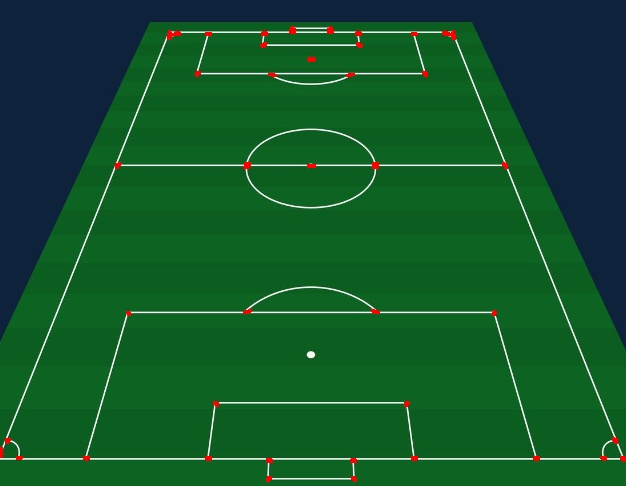
\includegraphics[width=0.3\textwidth]{Lab_3/template/figures/Harris_football.jpg}
    \caption{Ejemplo de detección de esquinas con el método Harris.}
    \label{fig:ejemplo_harris}
\end{figure}


\section*{Tarea A.5: Definición del método  Shi-Tomasi para detección de esquinas}
\addcontentsline{toc}{section}{Tarea A.5: Definición del método  Shi-Tomasi para detección de esquinas}
Defina la función \texttt{shi\_tomasi\_corner\_detection()}, que servirá para la detección de esquinas sobre las imágenes de trabajo. Siga los siguientes pasos:

\begin{itemize}
    \item Convertir la imagen de entrada a escala de grises utilizando \texttt{cv2.cvtColor()}.
    \item Aplicar el método \texttt{cv2.goodFeaturesToTrack()} \footnote{ \href{https://docs.opencv.org/3.4/dd/d1a/group\_\_imgproc\_\_feature.html\#ga1d6bb77486c8f92d79c8793ad995d541}{Documentación del método \texttt{goodFeaturesToTrack()} en OpenCV:} \\{https://docs.opencv.org/3.4/dd/d1a/group\_\_imgproc\_\_feature.html\#ga1d6bb77486c8f92d79c8793ad995d541}}.
    \item Convertir las coordenadas de las esquinas detectadas a enteros utilizando \texttt{np.intp}.
    \item Para cada esquina detectada, extraer las coordenadas \texttt{x} e \texttt{y} y dibujar un círculo en la imagen usando \texttt{cv2.circle()}.
\end{itemize}


\section*{Tarea A.6: Aplicación de Shi-Tomasi}
\addcontentsline{toc}{section}{Tarea A.6: Aplicación de Shi-Tomasi}
Aplique la función \texttt{shi\_tomasi\_corner\_detection()} sobre las imágenes de trabajo. Asegúrese de que las imágenes quedan guardadas como se especifica en los comentarios.

\section*{Preguntas}
\addcontentsline{toc}{section}{Preguntas}

\vspace{5mm}
\begin{tcolorbox}[colback=gray!10, colframe=gray!30, coltitle=black, title=Pregunta A.1, halign=left]
Realice la detección de esquinas en las otras dos imágenes de la carpeta \texttt{data/source} (cuyos nombres de guardado han de ser \textit{sudoku} y \textit{tennis}) con el método de Harris.
\end{tcolorbox}

\vspace{5mm}
\begin{tcolorbox}[colback=gray!10, colframe=gray!30, coltitle=black, title=Pregunta A.2, halign=left]
Realice la detección de esquinas en las otras dos imágenes de la carpeta \texttt{data/source} (cuyos nombres de guardado han de ser \textit{sudoku} y \textit{tennis}) con el método de Shi-Tomasi.
\end{tcolorbox}